\documentclass[letterpaper,12pt]{article}
\usepackage[dvips]{epsfig,geometry}
%\usepackage{multicol}
%\usepackage{fancyhdr}
%\pagestyle{fancy}
\usepackage{nicefrac}
\usepackage{indentfirst}
\usepackage{amssymb}
\usepackage{color}
\usepackage{enumerate}
\usepackage{comment}
\usepackage{overcite}
\usepackage{citesort}
\usepackage{geometry}
\usepackage{amsmath}
\usepackage[]{caption}
\usepackage{graphicx}
%\usepackage{aip}
\usepackage{bm}
\usepackage{wrapfig}
\usepackage{subfigure}

\usepackage{hyperref}

\geometry{letterpaper,textwidth=6.5in,textheight=9.0in,left=1.in,right=1in,top=1in}
\setlength{\parindent}{0.25in}
\renewcommand{\baselinestretch}{1.25}
\baselineskip = 13pt

\columnsep = 0.125in



%Definition of new commands
\newcommand{\f}[2]{\ensuremath{\frac{\displaystyle{#1}}{\displaystyle{#2}}}}
\newcommand{\lr}[1]{\langle{#1}\rangle}
\newcommand{\colv}[2] {\left(\begin{array}{c} #1 \\ #2 \end{array}\right)}
\renewcommand{\thefootnote}{\fnsymbol{footnote}}
\newcommand{\be} {\begin{eqnarray}}
\newcommand{\ee} {\end{eqnarray}}

%-------------------------------------------------------------------------------------------------------------------
%EQ COMMANDS
%-------------------------------------------------------------------------------------------------------------------

\newcommand{\two}{\mspace{-2.0mu}}
\newcommand{\four}{\mspace{-4.0mu}}
\newcommand{\plus}{\mspace{-4.5mu}+\mspace{-3.5mu}}
\newcommand{\minus}{\mspace{-4.5mu}-\mspace{-3.5mu}}
\newcommand{\pp}{'\mspace{-2.0mu}'}

\newcommand{\xlb}[4]{#1\ifthenelse{\equal{#2}{0}}{}{_{\alpha #2}}
\mspace{-2.0mu}\genfrac{(}{)}{0pt}{1}{\ifthenelse{\equal{#3}{0}}{0}{l #3}} {\ifthenelse{\equal{#4}{0}}{0}{b #4}}}

\newcommand{\xkv}[4]{#1\mspace{-5.0mu}\left(\mspace{-8.0mu}\begin{smallmatrix}#2\four{}\four{}\mspace{-8.0mu}&\pmb{\kappa}#3\\&\nu #4\end{smallmatrix}\mspace{-5.0mu}\right)}

\newcommand{\evect}[6]{#1\mspace{-4.0mu}\left(\mspace{-8.0mu}\begin{smallmatrix}#2\mspace{-8.0mu}&\pmb{\kappa} #3 &b #5\\&\nu #4 &\alpha #6\end{smallmatrix}\mspace{-5.0mu}\right)}

\newcommand{\varmat}[8]{\mspace{-5.0mu}\left(\mspace{-8.0mu}\begin{smallmatrix}\ifthenelse{\equal{#3}{0}}{\mspace{-8.0mu}&b_{#1}&b_{#2}\\&\alpha_{#1}&\alpha_{#2}} {\ifthenelse{\equal{#7}{0}}{#1\mspace{-8.0mu}&\pmb{\kappa}#2#3\mspace{-8.0mu}&\pmb{\kappa}#4#5\mspace{-8.0mu}&\pmb{\kappa}#6\\&\nu#2&\nu#4&\nu#6} {#1\mspace{-8.0mu}&\pmb{\kappa}#2#3\mspace{-8.0mu}&\pmb{\kappa}#4#5\mspace{-8.0mu}&\pmb{\kappa}#6#7\mspace{-8.0mu}&\pmb{\kappa}#8\\&\nu#2&\nu#4&\nu#6&\nu#8}}\end{smallmatrix}\mspace{-5.0mu}\right)}

\newcommand{\EXP}[1]{\exp\mspace{-5.0mu}\left[#1\right]\mspace{-3.0mu}}

\newcommand{\tpp}[2]{\left(\mspace{-2.0mu}\xkv{\omega}{}{}{}#1\xkv{\omega}{}{'}{'}#2\xkv{\omega}{}{\pp}{\pp}\mspace{-2.0mu}\right)}



\newcommand{\SUM}[2]{\ifthenelse{\equal{#1}{0}}{\sum_{\alpha_{#2},b_{#2},l_{#2}}^{3,n,N}} {\ifthenelse{\equal{#1}{1}}{\sum_{\alpha_{#2},b_{#2}}^{3,n}}{\sum_{\pmb{\kappa}#2,\nu#2}^{N,3n}}}}

\newcommand{\SUMprime}[2]{\ifthenelse{\equal{#1}{0}}{\sum_{\alpha_{#2},b_{#2},l_{#2}}^{3,n,N}} {\ifthenelse{\equal{#1}{1}}{\sum_{\alpha_{#2},b_{#2}}^{3,n}}{\sum_{\pmb{\kappa}^{'}#2,\nu#2}^{N,3n}}}}

\newcommand{\SUMalpha}[2]{\ifthenelse{\equal{#1}{0}}{\sum_{\alpha_{#2}}^{3}} {\ifthenelse{\equal{#1}{1}}{\sum_{\alpha_{#2},b_{#2}}^{3,n}}{\sum_{\pmb{\kappa}#2,\nu#2}^{N,3n}}}}

\newcommand{\SUMalphap}[2]{\ifthenelse{\equal{#1}{0}}{\sum_{\alpha'_{#2}}^{3}} {\ifthenelse{\equal{#1}{1}}{\sum_{\alpha'_{#2},b'_{#2}}^{3,n}}{\sum_{\pmb{\kappa}#2,\nu#2}^{N,3n}}}}

\newcommand{\SUMb}[2]{\ifthenelse{\equal{#1}{0}}{\sum_{b_{#2}}^{n}} {\ifthenelse{\equal{#1}{1}}{\sum_{\alpha_{#2},b_{#2}}^{3,n}}{\sum_{\pmb{\kappa}#2,\nu#2}^{N,3n}}}}

\newcommand{\SUMbp}[2]{\ifthenelse{\equal{#1}{0}}{\sum_{b'_{#2}}^{n}} {\ifthenelse{\equal{#1}{1}}{\sum_{\alpha'_{#2},b'_{#2}}^{3,n}}{\sum_{\pmb{\kappa}#2,\nu#2}^{N,3n}}}}

\newcommand{\SUMl}[2]{\ifthenelse{\equal{#1}{0}}{\sum_{l_{#2}}^{N}} {\ifthenelse{\equal{#1}{1}}{\sum_{\alpha_{#2},b_{#2}}^{3,n}}{\sum_{\pmb{\kappa}#2,\nu#2}^{N,3n}}}}

\newcommand{\SUMlp}[2]{\ifthenelse{\equal{#1}{0}}{\sum_{l'_{#2}}^{N}} {\ifthenelse{\equal{#1}{1}}{\sum_{\alpha'_{#2},b'_{#2}}^{3,n}}{\sum_{\pmb{\kappa}#2,\nu#2}^{N,3n}}}}

\newcommand{\abcdt}[5]{\mspace{-4.0mu}\left(\mspace{-8.0mu}\begin{smallmatrix}&\ifthenelse{\equal{#1}{}}{a}{#1}&\ifthenelse{\equal{#3}{}}{c}{#3}\\&\ifthenelse{\equal{#2}{}}{b}{#2}&\ifthenelse{\equal{#4}{}}{d}{#4}\end{smallmatrix}\mspace{-2.0mu};\ifthenelse{\equal{#5}{}}{t}{#5}\right)}

\newcommand{\abcd}[4]{\mspace{-4.0mu}\left(\mspace{-8.0mu}\begin{smallmatrix}&\ifthenelse{\equal{#1}{}}{a}{#1}&\ifthenelse{\equal{#3}{}}{c}{#3}\\&\ifthenelse{\equal{#2}{}}{b}{#2}&\ifthenelse{\equal{#4}{}}{d}{#4}\end{smallmatrix}\mspace{-3.0mu}\right)}

\newcommand{\abt}[3]{\mspace{-4.0mu}\left(\mspace{-8.0mu}\begin{smallmatrix}&\ifthenelse{\equal{#1}{}}{a}{#1} \\&\ifthenelse{\equal{#2}{}}{b}{#2}\end{smallmatrix}\mspace{-2.0mu};\ifthenelse{\equal{#3}{}}{t}{#3}\right)}

\newcommand{\ab}[2]{\mspace{-4.0mu}\left(\mspace{-8.0mu}\begin{smallmatrix}&\ifthenelse{\equal{#1}{}}{a}{#1} \\&\ifthenelse{\equal{#2}{}}{b}{#2}\end{smallmatrix}\mspace{-3.0mu}\right)}

\newcommand{\kvbat}{\mspace{-4.0mu}\left(\mspace{-8.0mu}\begin{smallmatrix} &\pmb{\kappa} &b \\ &\nu &\alpha\end{smallmatrix}\mspace{-2.0mu};t\right)}

\newcommand{\kvbatp}{\mspace{-4.0mu}\left(\mspace{-8.0mu}\begin{smallmatrix} &\pmb{\kappa} &b' \\ &\nu &\alpha'\end{smallmatrix}\mspace{-2.0mu};t\right)}

\newcommand{\kvbaw}{\mspace{-4.0mu}\left(\mspace{-8.0mu}\begin{smallmatrix} &\pmb{\kappa} &b \\ &\nu &\alpha\end{smallmatrix}\mspace{-2.0mu};\omega\right)}

\newcommand{\kvbawp}{\mspace{-4.0mu}\left(\mspace{-8.0mu}\begin{smallmatrix} &\pmb{\kappa} &b' \\ &\nu &\alpha'\end{smallmatrix}\mspace{-2.0mu};\omega\right)}

\newcommand{\kvba}{\mspace{-4.0mu}\left(\mspace{-8.0mu}\begin{smallmatrix} &\pmb{\kappa} &b \\ &\nu &\alpha\end{smallmatrix}\mspace{-3.0mu}\right)}

\newcommand{\kvbap}{\mspace{-4.0mu}\left(\mspace{-8.0mu}\begin{smallmatrix} &\pmb{\kappa} &b' \\ &\nu &\alpha'\end{smallmatrix}\mspace{-3.0mu}\right)}

\newcommand{\kpvba}{\mspace{-4.0mu}\left(\mspace{-8.0mu}\begin{smallmatrix} &\pmb{\kappa}^{'} &b \\ &\nu &\alpha\end{smallmatrix}\mspace{-3.0mu}\right)}

\newcommand{\kva}{\mspace{-4.0mu}\left(\mspace{-8.0mu}\begin{smallmatrix} &\pmb{\kappa} \\ &\nu &\alpha\end{smallmatrix}\mspace{-3.0mu}\right)}

\newcommand{\kvap}{\mspace{-4.0mu}\left(\mspace{-8.0mu}\begin{smallmatrix} &\pmb{\kappa} \\ &\nu &\alpha'\end{smallmatrix}\mspace{-3.0mu}\right)}

\newcommand{\kvb}{\mspace{-4.0mu}\left(\mspace{-8.0mu}\begin{smallmatrix} &\pmb{\kappa} &b \\ &\nu \end{smallmatrix}\mspace{-3.0mu}\right)}

\newcommand{\kvbp}{\mspace{-4.0mu}\left(\mspace{-8.0mu}\begin{smallmatrix} &\pmb{\kappa} &b' \\ &\nu \end{smallmatrix}\mspace{-3.0mu}\right)}

\newcommand{\kvt}{\mspace{-4.0mu}\left(\mspace{-8.0mu}\begin{smallmatrix}&\pmb{\kappa} \\&\nu\end{smallmatrix}\mspace{-2.0mu};t\right)}

\newcommand{\kpvt}{\mspace{-4.0mu}\left(\mspace{-8.0mu}\begin{smallmatrix}&\pmb{\kappa}^{'} \\&\nu\end{smallmatrix}\mspace{-2.0mu};t\right)}

\newcommand{\kvw}{\mspace{-4.0mu}\left(\mspace{-8.0mu}\begin{smallmatrix}&\pmb{\kappa} \\&\nu\end{smallmatrix}\mspace{-2.0mu};\omega\right)}

\newcommand{\kv}{\mspace{-4.0mu}\left(\mspace{-8.0mu}\begin{smallmatrix}&\pmb{\kappa} \\&\nu\end{smallmatrix}\mspace{-3.0mu}\right)}

\newcommand{\lbt}{\mspace{-4.0mu}\left(\mspace{-8.0mu}\begin{smallmatrix}&l \\&b\end{smallmatrix}\mspace{-2.0mu};t\right)}

\newcommand{\lbtp}{\mspace{-4.0mu}\left(\mspace{-8.0mu}\begin{smallmatrix}&l' \\&b'\end{smallmatrix}\mspace{-2.0mu};t\right)}

\newcommand{\lt}{\mspace{-4.0mu}\left(\mspace{-8.0mu}\begin{smallmatrix}&l\end{smallmatrix}\mspace{-2.0mu};t\right)}

\newcommand{\ltp}{\mspace{-4.0mu}\left(\mspace{-8.0mu}\begin{smallmatrix}&l'\end{smallmatrix}\mspace{-2.0mu};t\right)}

\newcommand{\lb}{\mspace{-4.0mu}\left(\mspace{-8.0mu}\begin{smallmatrix}&l \\&b\end{smallmatrix}\mspace{-3.0mu}\right)}

\newcommand{\lbp}{\mspace{-4.0mu}\left(\mspace{-8.0mu}\begin{smallmatrix}&l' \\&b'\end{smallmatrix}\mspace{-3.0mu}\right)}

%-------------------------------------------------------------------------------------------------------------------
%COMMANDS
%-------------------------------------------------------------------------------------------------------------------



\begin{document}

\begin{center}



\centering

\vspace{1.1in}

\LARGE Thermal Transport in Disordered Materials\Large

\vspace{1in} A thesis proposal by\\Jason M. Larkin\\
\vspace{1.1in}


\parbox[h]{4in}{\center{April 25, 2008\\224 Scaife Hall\\Department of
Mechanical Engineering\\Carnegie Mellon University}}

\thispagestyle{empty}
\end{center}
\vspace{2.in}
\parbox[b]{6.5in}{\noindent \underline{Thesis Committee}\\
\noindent Associate Professor Alan McGaughey (Committee Chair), Mechanical Engineering\\
Professor Jonathan A. Malen, Mechanical Engineering \\
Professor Michael Widom, Physics \\
Professor Craig Maloney, Civil and Environmental Enginering\\}

\clearpage

\tableofcontents

\clearpage

\section{\label{S-Intro}Introduction}

\subsection{\label{S-Intro}Thermal Transport in Ordered Materials}

1) Understanding thermal transport in crystalline systems requires detailed knowledge of the phonon properties.

Thermal transport in a semiconductor is controlled by phonons, quanta of energy associated with atomic vibrations. The properties of phonons are controlled at atomic-level length scales of 0.1-1 nm. Phonons themselves are non-localized vibrations which can extend over 100 nm – 10 microns in common semiconducting materials like silicon and germanium.  A nanostructured material can be described by an effective thermal conductivity, which can be very different than the bulk values available in common references.  The effective thermal conductivity of a nanostructure is lower than the bulk value due to the scattering of phonons with the system boundaries which have length scales of 10 nm – 100 microns.

\subsection{\label{S-Intro}Thermal Transport in Disordered Materials}


2) Thermal transport in dilute alloys should have significant contribution from phonons.  As the alloy concentration is increased, the vibrational modes should become localized and non-propagating.

1) Thermal transport in amorphous materials is typically modeled as completely localized vibrations which propagate diffusively.\cite{allen1993}  This diffusive propagation is much slower than the long-range propagation of phonons, and thus the thermal conductivity of amorphous materials is typically several orders of magnitude less than crystalline systems.\cite{freeman1986,cahill1992}

The first evidence of such localized modes, was reported by Keppens et al.\cite{keppens1998} using heat
capacity, elastic constant and inelastic neutron-scattering
measurements. They were able to explain their heat-capacity data with the Debye model plus two fitted Einstein oscillators. Recently there have been debates on this picture. It has
been pointed out by a higher resolution neutron scattering
that the previously observed peaks were due to van Hove
singularities, that is, optical phonons and zone boundary
modes.

1) Thermal transport in amorphous materials has AF theory, but recent measurements show that this theory
is incomplete because it does not consider the contribution from phonons to thermal transport.\cite{he2011} These modes are long wavelength and thus sample an effective medium of the underlying disordered atomic structure.

1) The AF theory of thermal transport in amorphous solids also does not consider the effects of anharmonicity, which will be inverstigated using a combination of MD and LD calculations.\cite{cahill1987}

1) what do ab initio structures/calculations predict for amorphous materials, such as silicon? Use DFT MD to produce amorphous structure(s). Use harmonic FC's to run classical MD and Green-Kubo.  Is it possible to accurately predict thermal conductivity using harmonic FCs for other disordered systems such as alloys?

Predicting and describing transport physics requires insight into
the movement and scattering of transport carriers. Transport
carriers include fluid molecules, electrons, and phonons (quantized
lattice vibrations) \cite{kaviany2008}. These carriers are what move
in response to spatial gradients and give rise to mass, momentum,
charge, and thermal energy fluxes through a system. The carriers
available for transport are directly related to the chemical
composition and thermodynamic phase of the host material. For
example, heat flux through crystalline solids is realized by phonons
(in an electrically insulating crystal) or electrons (in an
electrically conducting crystal). In an ideal gas, heat flux is
realized by elastic collisions between atoms and molecules.

\subsection{\label{S-Intro-Motivation}Large Unit Cell Materials for Thermoelectric Energy Generation}

Thermoelectric energy generation - the transformation of waste heat into useful electricity - is a promising source of sustainable energy \cite{ADMA:ADMA200600527}. Thermoelectric materials directly convert temperature differences into electric voltage as a result of their intrinsic (atomic-level) electronic and thermal properties. The performance of a thermoelectric device can be quantified through the thermoelectric figure of merit, ZT = , where T is the average device temperature, S is the Seebeck coefficient (the ratio of the induced thermoelectric voltage to the applied temperature difference),  is the electrical conductivity, and  is the thermal conductivity.  For thermoelectric devices to be competitive with traditional power generation cycles requires ZT > 3 \cite{Chen_Dresselhaus_Dresselhaus_Fleurial_Caillat_2003}. Achieving this performance is challenging because the electrical and thermal properties in ZT are coupled in the majority of materials \cite{ADMA:ADMA200600527,Chen_Dresselhaus_Dresselhaus_Fleurial_Caillat_2003}. The ideal thermoelectric can be thought of as an “electron-crystal/ phonon-glass” (high , low ) (see Figure 1). Reducing  has become a primary strategy in the design of new thermoelectric materials \cite{ADMA:ADMA200600527}.  Using nanostructuring to reduce  while maintaining good electrical properties has been identified as one possible strategy \cite{B822664B}, but such materials are costly. An emerging area of study in thermoelectric power generation is the use of large unit cell (LUC) crystals \cite{ADMA:ADMA200600527}.

 Large unit cell crystals have an ordered (crystalline) structure, but the basic building block (unit cell) of the crystal has a large number of distinct atoms (Figure 1) \cite{cm052055b,Yang_Chen_2006,wang_232107}.  They are effectively disordered over length scales on the order of the atomic spacing and their thermal conductivities can be as low as a glass \cite{cm052055b,Yang_Chen_2006,wang_232107}. The key advantage of LUC materials is that they are still ordered from the standpoint of electrons, which results in large  and ZT. Thus, LUC crystals are “electron-crystal/phonon-glass” materials. Current LUC crystals have ZT<3 \cite{cm052055b,Yang_Chen_2006,wang_232107} and more research is required to improve their thermoelectric performance. 
The LUC crystals to be studied here are skutterudites \cite{cm052055b} and Zintl compounds \cite{wang_232107} (Figure 2). Both of these LUC crystals have , but experimental measurements show intriguing potential for improved thermoelectric efficiency \cite{cm052055b,Yang_Chen_2006,wang_232107}.  


\textit{It is
likely that the thermoelectric performance of large unit cell materials has yet to be fully realized.}

\subsection{\label{S-Intro-Motivation} Zeolites for Gas Adsorbation }

The porous crystals are a diverse group of materials
characterized by large unit cells and Angstrom sized pores
and channels. Among these are the zeolites [1], skutteru-
dites [2], fullerenes [3], and metal organic frameworks
[4,5]. The size of the pores is on the same scale as the
dimensions of many atoms and molecules, leading to the
use of porous crystals as molecular sieves and catalysts,
and for gas storage applications.

There is also
interest in the design of porous crystals with very low
thermal conductivities for applications as rigid insulators
and to protect stored gases from ambient temperature
fluctuations. As a first step towards design for thermal
properties, the mechanisms by which heat is transferred
in these materials must be understood. Here, this goal
is pursued in the context of the zeolites.

Which phonons/vibrational modes are affected by the adsorbed gas molecules?  Cite Thomas CNT/water study for possible scattering.  In these zeolite systems, modes may not be phonons.  Possibly need to study  the time scale you can extract from the AF calculation.

\subsection{\label{S-Intro-Motivation} Amorphous Materials }

Amorphous materials are used in a number of applications:

\begin{itemize}

\item Amorphous silicon solar cells

\item amorphous silicon/silica substrates for various applications

cite measurements of anomlalous high amorphous thin film conductivity

\item amorphous metals, which are most likely still dominated by electron thermal/electrical transport.

\end{itemize}

\subsection{\label{S:Intro-Research-Plan}Research Plan}

The objectives of the proposed research are to:

\begin{itemize}
\item Investigate thermal transport in crystals, alloys, and amorphous samples using model LJ systems. 

\item Develop methodology to identify relative contribution to thermal transport from thermal diffusivities in these systems.  

\item Design and perform ab initio simulations to predict the thermal properties of realistic LUC crystals. 

\end{itemize}

\section{\label{S:Intro-Review}Thermal Transport in Ordered and Disordered Materials}

\subsection*{\label{S:Thermal-Transport-Conductivty}Thermal Conductivity in Ordered Materials}
 
\begin{equation}\label{EQ:M:k_thermal}
k_{thermal} =\& k_{elec} + k_{lattice} 
			=\& k_{lattice}
\end{equation}

\begin{equation}\label{EQ:M:k_thermal}
k_{elec} = 
\end{equation}

%\url{http://hyperphysics.phy-astr.gsu.edu/hbase/thermo/thercond.html#c2}
%\href{http://hyperphysics.phy-astr.gsu.edu/hbase/thermo/thercond.html#c2}{elec_cond}
%
%\url{http://en.wikipedia.org/wiki/Electron_mobility}
%\href{http://en.wikipedia.org/wiki/Electron_mobility}{elec_mobility}


Making no assumptions about the phonons, the lattice thermal conductivity is given as a sum over all phonon modes with mode specific properties

\begin{equation}\label{EQ:k_sum}
\begin{split}
k_{lattice,\mathbf{n}}=&\sum_{\pmb{\kappa}} \sum_\nu c_{ph} \kv v^{2}_{g,\mathbf{n}} \kv \tau \kv.
\end{split}
\end{equation}

Taking the specific heat to be $c_{ph} \kv = k_{B}$, the thermal conductivity is 

\begin{equation}\label{EQ:k_sum}
\begin{split}
k_{lattice,\mathbf{n}}=&\sum_{\pmb{\kappa}} \sum_\nu k_{B} D \kv.
\end{split}
\end{equation}

And the thermal conductivity is determined by the phonon mode diffusitivies,

\begin{equation}\label{EQ:k_sum}
\begin{split}
D \kv =  \kv v^{2}_{g,\mathbf{n}} \kv \tau \kv.
\end{split}
\end{equation}

Using the Debye model, the thermal conductivity can be re-written

\begin{equation}\label{EQ:k_sum}
\begin{split}
k_{lattice}=& \frac{1}{3} \int_{0}^{\omega_{D}} C(\omega) D_{p}(\omega) d\omega.
\end{split}
\end{equation}

\begin{equation}\label{EQ:k_sum}
\begin{split}
D_{p}(\omega) =  v^{2}(\omega) \tau(\omega).
\end{split}
\end{equation}


\subsection{\label{S-validation-samples}Phonon Lifetimes and Scattering Mechanisms}


\begin{equation}\label{EQ:M:tau_matthiessen}
\frac{1}{\tau} = \frac{1}{\tau_{p-p}} + \frac{1}{\tau_{b}} + \frac{1}{\tau_{d}}
\end{equation}

\begin{equation}\label{EQ:M:tau_p-p}
\tau_{p-p} = (6 \pi^2)^(1/3)/2 Mavg v_g v_p^2 / V^1/3 \omega^2 \gamma^2 T
\end{equation}

\begin{equation}\label{EQ:M:tau_b}
\tau_{b} = L/v_g
\end{equation}

\begin{equation}\label{EQ:M:tau_d}
\tau_{d} = \frac{V \omega^4}{4 \pi v_p^2 v_g} ( \sum_i c_i(1-m/\bar(m_i))^2 + \sum_i c_i(1-r/\bar(r_i))^2 )
\end{equation}


\section*{Thermal Conductivity in Disordered Materials}

\subsection{\label{S-validation-samples}Phonons in Disordered Materials}

\subsection{\label{S-validation}Dilute Alloys}


\begin{equation}\label{EQ:M:k_thermal}
k_{lattice} = k_{phonon}
\end{equation}

\begin{equation}\label{EQ:M:tau_d}
\tau_{d} = \frac{V \omega^4}{4 \pi v_p^2 v_g} ( \sum_i c_i(1-m/\bar(m_i))^2 + \sum_i c_i(1-r/\bar(r_i))^2 )
\end{equation}

Phonons still dominate the transport:

\begin{equation}\label{EQ:M:tau_matthiessen}
\frac{1}{\tau} = \frac{1}{\tau_{p-p}} + \frac{1}{\tau_{b}} + \frac{1}{\tau_{d}}
\end{equation}


\subsection{\label{S-validation}High Concentration Alloys and Glasses}

Alan 2004 IJMHT amorphous silica shows increasing k with T in classical system, not a heat capacity effect.

\begin{equation}\label{EQ:M:k_thermal}
k_{lattice} = k_{phonon} + k_{AF}
\end{equation}

\begin{equation}\label{EQ:M:k_thermal}
k_{AF} = \sum_i C(\omega_i)_{i} D(\omega_i)_{i} 
\end{equation}

Given Fig. \ref{F:phonon_diff}, how can we differentiate between phonons and AF modes?  Galli says it's when the phonon mean free path is on the order of the atomic spacing.  However, it seems more appropriate to consider the AF or phonon mode diffusivities.  For example, some phonon modes have a finite lifetime, but vanishing group velocities.   

\begin{figure}
\begin{center}
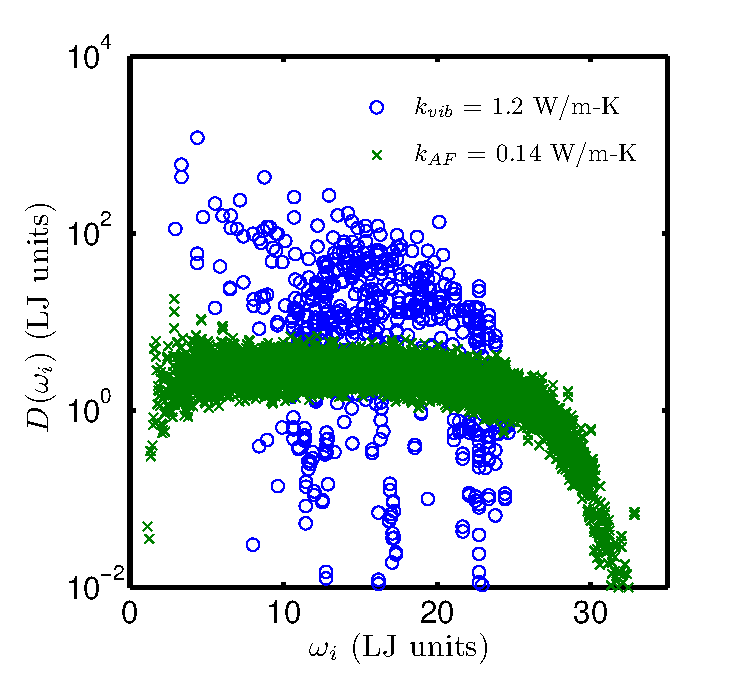
\includegraphics[scale=0.5]{phonon_diff.eps}
\vspace*{-5mm}
\end{center}
\caption{\label{F:phonon_diff} plot comparison of phonon diffusivity versus AF mode diffusivity for LJ 4x.}
\end{figure}

Cahill\cite{PhysRevB.46.6131} suggests that the phonon mean free paths in glasses scales as the wavelength of the mode:

\begin{equation}\label{EQ:M:l_glass}
l_{glass} =  \lambda /2
\end{equation}

This length scale is still much larger than atomic spacings! Galli suggests that the differentiation between phonon and AF modes is when the phonon mean free path is on the order of the atomic spacings. 

Cahill model leads to following scaling of lifetimes in glasses\cite{PhysRevB.46.6131}

\begin{equation}\label{EQ:M:l_glass}
\tau_{glass} =  \pi frac{p}{\omega}
\end{equation}

Hypothesis:

May be more likely that the low frequency acoustic phonons in glasses follow a Debye model with Umklapp scattering:

\begin{equation}\label{EQ:M:tau_p-p}
\tau_{p-p} = (6 \pi^2)^(1/3)/2 Mavg v_g v_p^2 / V^1/3 \omega^2 \gamma^2 T
\end{equation}

Under this hyopthesis, the lattice thermal conductivity from phonons is

\begin{equation}\label{EQ:M:k_thermal}
k_{phonon} = \frac{(6 \pi^2)^(2/3)}{4 \pi^2} \frac{ Mavg v_s^3}{ V^{2/3} \omega^2 \gamma^2 T}
\end{equation}

Which can be accounted for using Lattice Dynamics.  If this result for the phonon contribution can be combined with the AF contribution, then disordered materials can characterized solely from (harmonic) lattice dynamics which is computationally inexpensive (see Appendix \ref{}).


\subsubsection{\label{S-MD-SW}AF Lifetime}

Using dimensional analysis, the thermal diffusivity calculated by the AF theory can possibly be decomposed into a velocity and time scale:

\begin{equation}\label{EQ:M:k_thermal}
D(\omega_i)_{i} = v^2_{AF} \tau_{AF}
\end{equation}




\vspace*{25mm}






\clearpage

\section{\label{S-Intro-Dispersion_Disordered} Controlling Thermal Transport in Disordered Materials}

\subsection{\label{S-Intro-Dispersion_Disordered}Controlling Thermal Transport by Dispersion}

Controlling dispersion through 

\begin{itemize}

\item mass ratio

k is dramatically overestimated
by the Debye model when mass
contrast is high (e.g. BaO, mass ratio
of 8.6).\cite{Toberer2011}

when limited by Umklapp scattering, the
spectral thermal conductivity, $ks(\omega)$, is
proportional to $vg(\omega)^2$.

The relationship between mass contrast and k can be understood by examining
the BvK phonon dispersions for a diatomic chain with varying mass ratio,
m1/m2. When the mass ratio is low, the Debye model assumption of
a constant phonon velocity is reasonable. However, this assumption breaks down as the mass ratio increases and the optical branch flattens.  \cite{PhysRev.141.767} 

\item Numer of atoms in unit cell

\begin{figure}\begin{center}
\caption{\label{F:PEAK_COMPARE} Plot [100] dispersion w(k,c=0..0.5) showing $\bf{effective mass}$ effect and N effect}
\end{center}\end{figure}

Generically folds the dispersion branches in, decreasing both acoustic group velocities and flattening optical branches.

\item amorphization

\begin{figure}\begin{center}
\caption{\label{F:PEAK_COMPARE} Plot [100] dispersion of 4x crystal using supercell definition, c=0.5, amorphous}
\end{center}\end{figure}

Amorphous sample should be lower coordinated than crystal.  This will make the sample bulk modulus smaller, which should lead to a smaller sound speed (acoustic group velocity):

\begin{equation}\label{E-Seq}
v_s = \sqrt{B_{glass}/\rho}
\end{equation}

\end{itemize}

\begin{figure}
\begin{center}
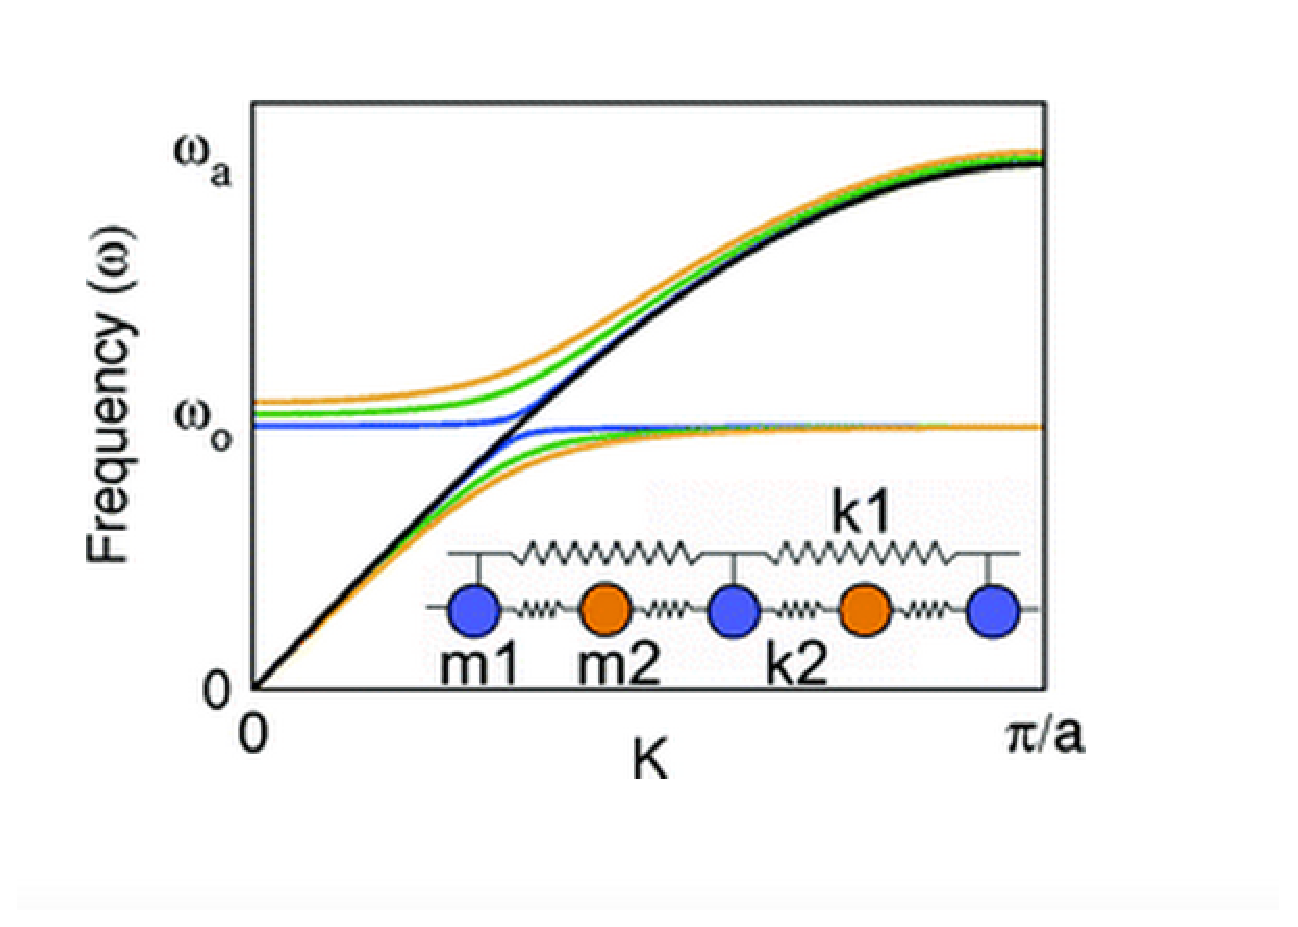
\includegraphics[scale=0.5]{flat_dispersion.eps}
\vspace*{-5mm}
\end{center}
\caption{\label{F:PEAK_COMPARE} flattening of dispersion .}
\end{figure}

\begin{figure}
\begin{center}
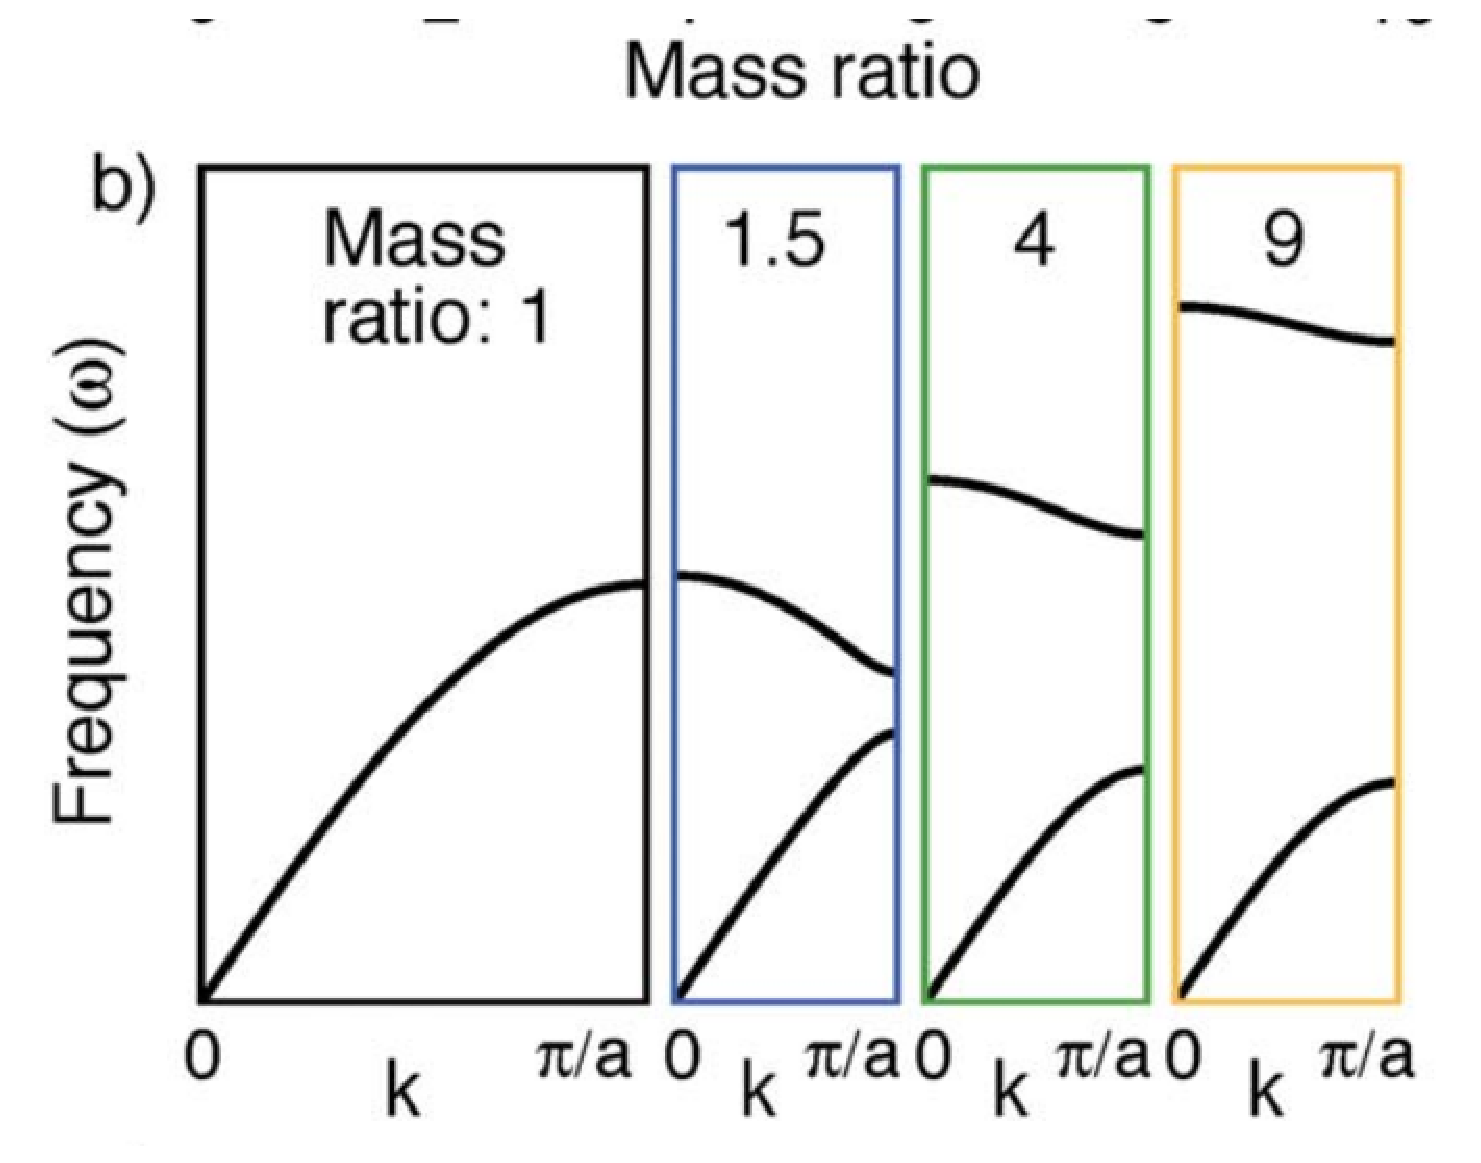
\includegraphics[scale=0.5]{vg_mass_ratio.eps}
\vspace*{-5mm}
\end{center}
\caption{\label{F:PEAK_COMPARE} The phonon spectral energy density ($\Phi$) .}
\end{figure}


\subsection{\label{S-validation-samples}Implications for LUC}

\begin{itemize}

\item Mass Ratios in Diatomic Alloy such as PbTe, Bi2Te3, etc.

\item Number of atoms in unit cell effect on group velocity

As b increases, the
phonon dispersion ‘‘folds in’’ on itself,
resulting in b-1 optical modes with low
$v_g$.

Specifically, the breakdown of the $k = b^{-2/3}$ (Umklapp dominated) or $k = b^{-1}$ (boundary scattering dominated) scalings need to be investigated. This implies that sub-unit cell effects are important since the scalings rely on phonons to develop those scalings. 

\end{itemize}

%\begin{figure}
%\begin{center}
%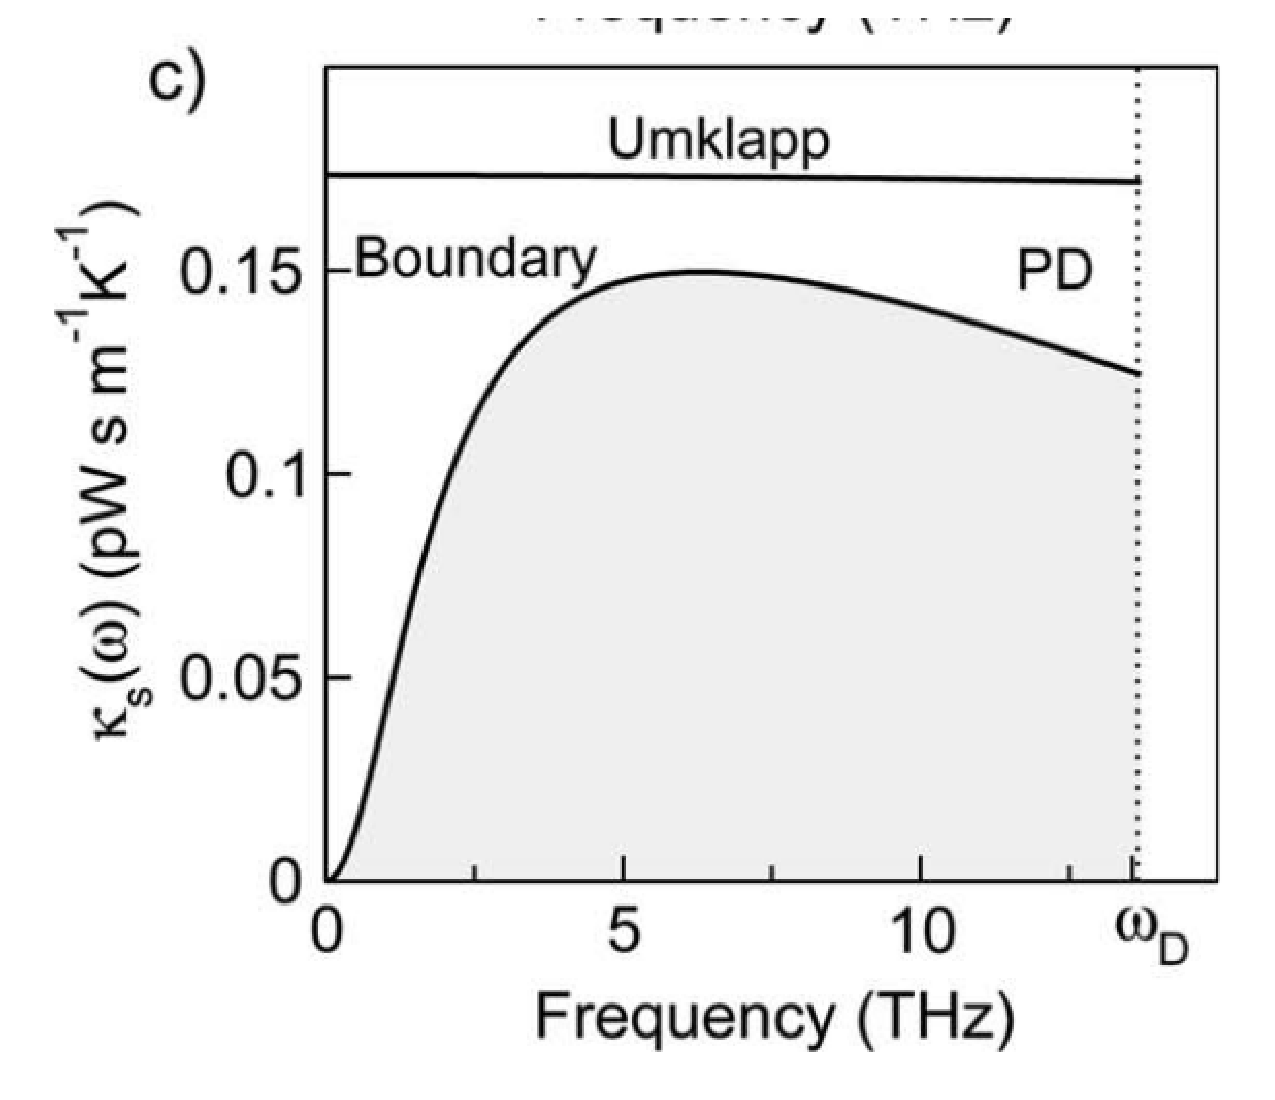
\includegraphics[scale=0.5]{k(w)_umklapp_boundary_PD.eps}
%\vspace*{-5mm}
%\end{center}
%\caption{\label{F:PEAK_COMPARE} Spectral thermal conductivity including all contributions (phonon-phonon, point defect, AF modes.}
%\end{figure}


\subsection{\label{S-Intro-Dispersion_Disordered}Controlling Thermal Transport by Thermal Diffusivity}


\begin{figure}
\begin{center}
\vspace*{-5mm}
\end{center}
\caption{\label{F:PEAK_COMPARE} NMD unit cell projection c=0..0.15
4x-6x-8x-10x. NMD full cell projection c=0.15 and 0.5  
4x-6x-8x-10x. }
\end{figure}



\begin{equation}\label{EQ:M:l_glass}
D_{p} =  \tau{p-p}v^2_{g}
\end{equation}

Boundary scattering attacks the low frequency/long wavelength modes, defect scattering attacks the high frequency/short wavelength, and Umklapp scattering attacks the mid-low frequency/intermdiate wavelength modes.

AF modes have much smaller diffusivity than the dominant diffusivities above (when present):

\begin{equation}\label{EQ:M:l_glass}
D_{AF} =  \tau{AF}v^2_{AF}
\end{equation}

In other words, the design strategy is to minimize the other diffusivities and so that only $D_{AF}$ remain.  How are the $D_{AF}$ controlled?

\begin{itemize}

\item bonding/coordination.  This may be where the Si02 measurements can come in

\item quench rates, etc.  Do not want to investigate this.

\item nanostructuring to beat the "amorphous limit", WSe2, etc.

\end{itemize}

\subsection{\label{S-validation-samples}Thermal Diffusivity Implications for LUC}

\subsubsection{\label{S-validation-samples}b=$\infty$ Large Unit Cells and Allen Feldman Modes}

At the amorphous limit ($N = \infty$), the acoustic contribution (ka) approaches
zero, whereas in practice, glasses still possess finite thermal conductivity.

Clearly, we cannot completely ignore the thermal conductivity of the optical modes in which most of the heat in a complex solid is stored. As a lower bound to the optical contribution to thermal conducivity (ko), one can look to Einstein’s treatment of heat transport as the diffu-
sion of heat between atomic oscillators.

Cahill 

\begin{equation}\label{EQ:M:l_glass}
l_{glass} =  \lambda/2,
\end{equation}

This is still much larger than distance between atoms! \cite{ascroft} Allen Feldman modes are $D_{i}$ 

Cahill model leads to following scaling of lifetimes in glasses\cite{PhysRevB.46.6131}

\begin{equation}\label{EQ:M:l_glass}
\tau_{glass} =  \pi frac{p}{\omega}
\end{equation}

How do these models agree in limits? Why is this a good model, because it fits data? This represents a clear difference between theoritical and empirical modeling. Does amorphous NMD calculate phonons with lifetimes which follow this trend?  If not, then this model's only purpose is to provide fitting parameters to fit empirical data.



\section{\label{S-validation}Large Unit Cell Materials}

\subsection{\label{S-validation-samples}SiO2}

How is this a model system for LUC?  

Is it based on N=small, but many configurations.  The different configurations must give different thermal conductivities.  Quantify phonons and AF contributions. 

Show that there is more scattering for some given coordiantions, indicating the importance of bonding/coordination in a control system.  If this is true, should be able to show this in an AF calculation in therms of the diffusivities.  

Might be alot easier to show this than do a phonon calculation.

Denisty probably changes though, so figure out a way to possibly collapse the data. 

\subsection{\label{S-validation-samples}Skutterudite Materials}

List the design strateiges presented above which can study these systems:


\begin{figure}
\begin{center}
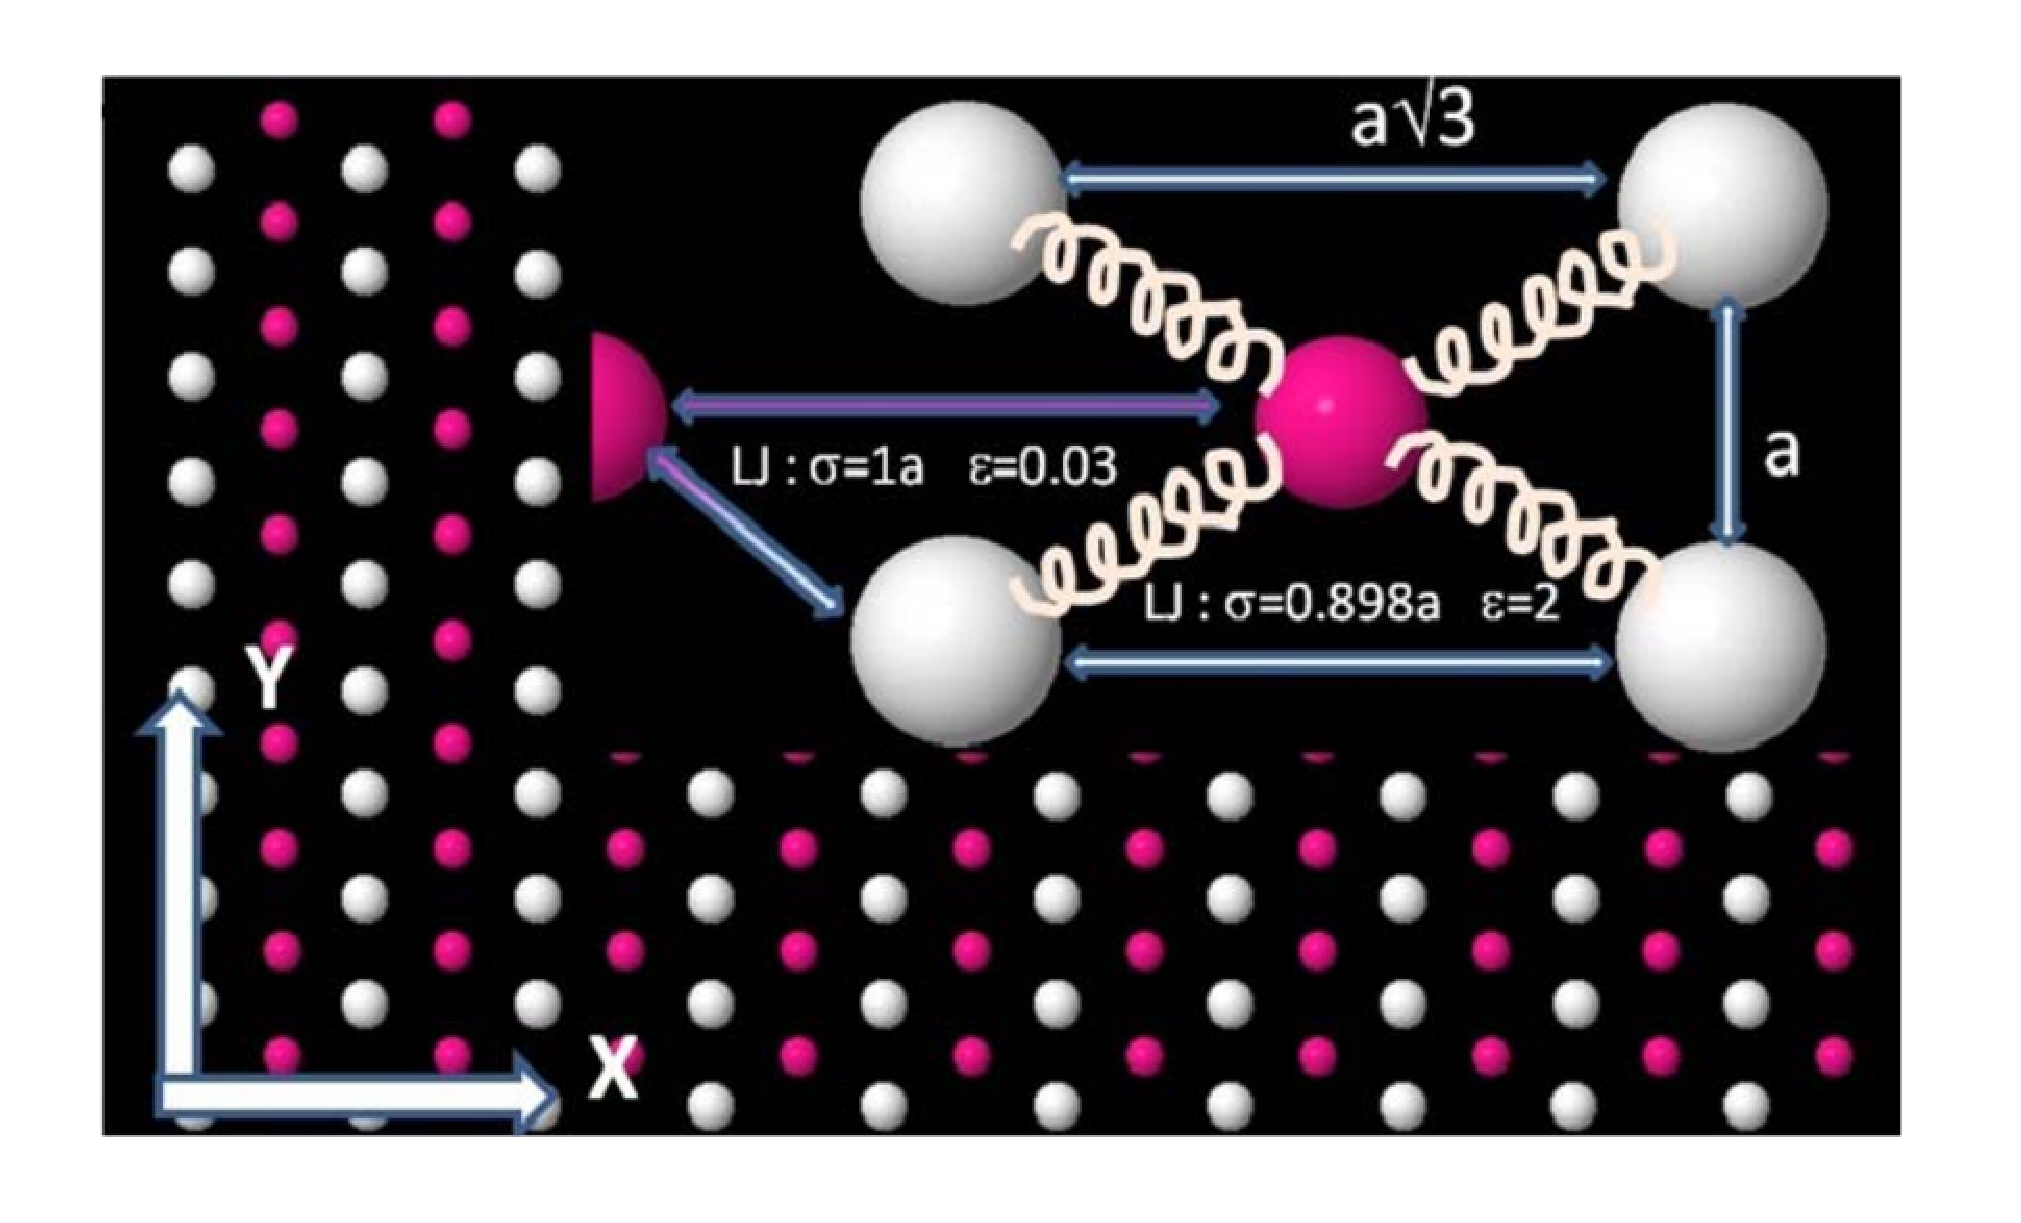
\includegraphics[scale=0.25]{skutt_lj_model.eps}
\vspace*{-5mm}
\end{center}
\caption{\label{F:PEAK_COMPARE} The phonon spectral energy density ($\Phi$) .}
\end{figure}

\subsubsection{\label{S-validation-samples}Rattling Modes}

Much of the excitement surrounding
skutterudites and clathrates has been
focused on the prediction66 and observa-
tion of a phenomena termed
‘‘rattling’’, observed when the guest atom
is under-constrained and weakly bound.\cite{keppens1998,Sales_Chakoumakos_Mandrus_Sharp_1999,doi:10.1021/ja063695y}

Experimentally, materials in which guest
atoms are strong rattlers are found to
exhibit extremely low kL.\cite{Sales_Chakoumakos_Mandrus_Sharp_1999,qiu:063713} While it is
widely accepted that rattling atoms result
in strongly localized modes within the
acoustic frequency range, the mechanism
by which rattler modes reduce kL is under
debate.

The reduction in kL
has been attributed to resonant scattering
by the guest atom.\cite{PhysRevLett.82.779} However, the impact
of rattling on the group velocity has
recently been recognized as an alternative
explanation of the low experi-
mental kL.\cite{Yang_Chen_2006,Christensen2008}

used to explain the unusual temperature
dependence of kL for both clathrates and
skutterudites.71,76 However, these models
assume a constant group velocity, which
fails to capture the complexity of the
phonon dispersion and the interaction of
the rattling and acoustic modes.


Fleurial et al.2 experimentally showed that the thermal conduc-
tivity decreases exponentially as the atomic-displacement
parameter increases.18

18
C. Godart, A. P. Gonçalves, E. B. Lopes, and B. Villeroy, Prop-
erties and Applications of Thermoelectric Materials ͑Springer,
Netherlands, 2009͒.

\subsection{\label{S-Intro-Motivation} Zeolites for Gas Adsorbation }



\clearpage

\section{\label{S-summaryschedule}Outcomes and schedule}

The outcomes of this proposed research will be:

\begin{itemize}

\item Characterization of Thermal Transport in Disordered Materials using LJ Models

\item Investigation of Thermal Transport in Large Unit Cell Materials

\item Investigation of Harmonic and Anharmonic Contributions to Thermal Transport in Disordered Materials

\item Computational Cost Analysis of Harmonic and Anharmonic Calculations

\item Detailed Computational Framework


\end{itemize}

The schedule for my proposed research is provided in Table:


\begin{tabular}{l*{6}{c}r}
Task              				& Fall 2011 & Winter 2012 & Spring 2012  \\
\hline
Characterization of Disordered LJ Models 	& --------- & --------- &  \\
Investigate Harmonic and Anharmonic Contributions	&  &  & --------- \\
\hline
Task  							& Summer 2012 & Fall 2012  & Winter 2013 \\
\hline
Investigate Transport in LUC 	& --------- & ---------   &  \\
Investigate Transport in LUC using Ab-Initio	& & & --------- \\
Investigate Harmonic and Anharmonic Contributions & & & --------- \\
\hline
Task  							& Spring 2013 & Summer 2013 & \\
\hline
Si amorphous study using Ab-Initio  & --------- & & \\	
Deliver thesis					& & --------- & --------- \\						
\end{tabular}

\vspace{1cm}

%\begin{figure}[h]
%\centerline{\epsfig{figure=timeline2.eps}}
%\caption{\label{fig:timeline2} \small{Research timeline.}}
%\end{figure}

\clearpage

\section{Biographical Sketch} 
Jason Larkin was born in Monroeville, PA.  He obtained his Bachelor's of Science degree
in mechanical engineering from the University of Pittsburgh in
Spring 2007. He obtained his Master's of Science degree in mechanical engineering in summer 2009 with a thesis: Statistics of Particle Concentrations in Free-Surface Turbulence. He entered Carnegie Mellon in Fall 2009 where he is pursuing his PhD in mechanical engineering.

\section*{\label{S-awards}Awards}

Northrop-Grumann Fellow, CIT Institute for Complex Engineered Systems (ICES) 2011

NSF Graduate Student Research Grant, University of Pittsburgh Department of Physics 2007-2009

2011 Bennett Presentation (Award for Best Presentation).

October 2011 Cover article for Physics of Fluids.

\section*{Peer-reviewed Journal Publications}

\begin{itemize}

\item “Predicting Phonon Properties of Silicon from First -Principles Calculations”, A. Jain, J.M. Larkin, A.J.H.
McGaughey, W.A. Al-Saidi, in preparation.

\item “Predicting Phonon Properties of Disordered Systems”, J.M. Larkin, A.J.H.
McGaughey, Ankit Jain, in preparation.

\item S. Stefanus, J. Larkin, W. Goldburg, “A Search for Conformal Invariance in Compressible Two
Dimensional Turbulence”, Physics of Fluids 23 (2011) 105101. Selected for cover.

\item J. Larkin, W. Goldburg, M.M. Bandi, “Time-Evolution of a fractal distribution: Particle concentrations
in free-surface turbulence”, Physica D 239 14 (2010) 1264-1268.

\item J. Larkin, W. Goldburg, “Decorrelating a Compressible Turbulent Flow: an Experiment”, Physical Review E
82, 016301 (2010).

\item J. Larkin, M.M. Bandi, A. Pumir, W. Goldburg , “Power -law distributions of particle concentration in
free-surface flows”, Physical Review E 80, 066301 (2009).

\end{itemize}

\section*{Conference Presentations}

\begin{enumerate}


\item “Predicting Phonon Properties of Silicon from First -Principles Calculations”, J.M. Larkin, A.J.H.
McGaughey, W.A. Al-Saidi, to be presented at 2012 ASME Summer Heat Transfer Conference Puerto
Rico, USA.

\item “Comparison of Spectral Energy Methods for Predicting Phonon Properties”, J.M. Larkin, A.D.
Massicotte, J.E. Turney, C.H. Amon, A.J.H. McGaughey, to be presented at 2012 ASME
Micro/Nanoscale Heat \& Mass Transfer International Conference Atlanta, GA.

\item “Predicting Thermal Conductivity of Defected Systems using the Spectral Energy Density”, J. Larkin
2011 MRS Fall Meeting Boston, MA.

\item “Predicting Thermal Conductivity of Defected Systems using the Spectral Energy Density”, J. Larkin
2011 Bennett Presentation (Award for Best Presentation).

\item “Decorrelating a Compressible Turbulent Flow: An Experiment”, J. Larkin, W. Goldburg (speaker),
2010 American Physical Society March Meeting Portland, OR.

\item “Statistics of Preferential Particle Concentration in Free -Surface Turbulence”, J. Larkin (speaker),
M.M. Bandi, W. Goldburg, 2009 American Physical Society March Meeting Pittsburgh, PA.

\item “Experimental Determination of the von Karman Constant in Turbulent Two Dimensional Soap Film
Flows”, Nicholas Guttenberg (speaker), Nigel Goldenfeld, Jason Larkin, Alisia Prescott, Hamid Kellay,
Walter Goldburg, 2008 Meeting of the APS Division of Fluid Dynamics San Antonio, TX.

\item “Turbulent Dynamics of a Hydraulic Jump in two dimensions: Soap Film Flow” Jason Larkin (speaker),
Walter Goldburg, Tuan Tran, Pinaki Chakraborty, Gustavo Goia, 2008 Meeting of the APS Division of
Fluid Dynamics San Antonio, TX.

\item “The Generalized Fractal Dimensions of a 2 -D Compressible Turbulence”, J. Larkin (speaker), M.M.
Bandi, W. Goldburg, 2008 American Physical Soci ety March Meeting New Orleans, LA.

\item “Design of a Flow Chamber to Explore the Initiation and Development of Cerebral Aneurysms”,
Jason Larkin, John P. Barrow, A. M. Robertson 2007 Biomedical Engineering Society Meeting
Undergraduate Presentation Los Angeles, CA


\end{enumerate}


\section{\label{S-validation}MISC}

For LUC systems, are the barriers more important than the crystallinity?

2) Rigidity-percolation models?

Feng Sen, Sahini
Thorpe, Duxbury
Boolchand

a) can you just run a harmonic FC MD to measure the conductivity?



\appendix

\section*{Lattice Dynamics}

\subsection{\label{S-MD-SW}Crystal Energy}

expansion of the crystal energy to motivate

\subsubsection{\label{S-MD-SW}Lennard-Jones Potential}

possibly present LJ, comment that it is simple but anharmonic

\subsection{\label{S-MD-SW}Harmonic Approximation and Normal Modes}

Show the dynamical matrix, here is where you get eigenvectors/freqs.

\subsection{\label{S-Intro-Review}Normal Modes in Ordered Solids}

start with the real space atomic velocities as represented by the normal mode decomposition,

\cite{dove1993}
\begin{equation}\label{E:udot_HLD}
\begin{split}
\dot{u}_{\alpha}\lbt = &\SUMprime{2}{} \frac{1}{\sqrt{m_bN}} \EXP{i\pmb{\kappa}^{'}\cdot\mathbf{r}_0\ab{l}{0}} e^*\kpvba \dot{q}\kpvt{}{}{}.
\end{split}
\end{equation}

\subsection{\label{Subsection_Comp_Details_1}Phonon Lifetimes from Normal Mode Decomposition}

Can get:

\begin{equation}\label{EQ:M:tau_p-p}
\tau_{p-p} = (6 \pi^2)^(1/3)/2 Mavg v_g v_p^2 / V^1/3 \omega^2 \gamma^2 T
\end{equation}

and for dilute alloys:

\begin{equation}\label{EQ:M:tau_d}
\tau_{d} = \frac{V \omega^4}{4 \pi v_p^2 v_g} ( \sum_i c_i(1-m/\bar(m_i))^2 + \sum_i c_i(1-r/\bar(r_i))^2 )
\end{equation}

\subsection{\label{Subsection_Comp_Details_1}Allowed Wavevectors in Ordered Systems}

The phonon spectral energy is defined for the allowed wavevectors of a crystal, which can be specified from the crystal structure's Bravais
lattice and its basis, i.e. unit cell. A $D$-dimensional Bravais lattice is a collection of points with
positions
\begin{equation}\label{crys_pos}
\begin{split}
\mathbf{r}_0\ab{l}{0} =& \sum^D_{\alpha} N_{\alpha}\mathbf{a}_{\alpha}
\end{split}
\end{equation}
where $N_{\alpha}$ and the summations if over the lattice vectors, $\mathbf{a}_{\alpha}$.\cite{ashcroft1976} The basis (or unit cell) is the building block of the crystal and they are arranged on the points defined by the Bravais lattice. The equillibrium position of any atom in the crystal can be described by
\begin{equation}\label{crys_pos2}
\begin{split}
\mathbf{r}_0\ab{l}{b} = \mathbf{r}_0\ab{l}{0} + \mathbf{r}_0\ab{0}{b}
\end{split}
\end{equation}
where $\mathbf{r}_0\ab{l}{0}$ and $\mathbf{r}_0\ab{0}{b}$ are the equilibrium positions of the $l^{\textrm{th}}$ unit cell and $b^{\textrm{th}}$ atom in the unit cell, respectively.

The allowed wavevectors are defined by
\begin{equation}\label{crys_pos3}
\begin{split}
\pmb{\kappa} = \sum_{\alpha} \mathbf{b}_{\alpha} \frac{n_{\alpha}}{N_{\alpha}}
\end{split}
\end{equation}
where $\mathbf{b}_{\alpha}$ are the reciprocal lattice vectors\cite{ashcroft1976}, which are related to the (Bravais) lattice vectors in Eq$.$ \ref{crys_pos}, and $-N_{\alpha}/2 < n_{\alpha} \leq N_{\alpha}/2$, where $n_{\alpha}$ and $N_{\alpha}$ are even integers.\cite{turney2009a} The reciprocal points are taken to be in the first BZ.\cite{ashcroft1976}


\subsubsection*{Allowed Wavevectors in Disordered Materials}

Strictly speaking, the only allowed wavector in a disordered system is the gamma point. As such, the lattice dynamics calculations are performed at the gamma point:

\begin{equation}\label{crys_pos3}
\begin{split}
\omega^2 \kv \mathbf{e} \kv = D \kv \mathbf{e}
\end{split}
\end{equation}

\begin{equation}\label{crys_pos3}
\begin{split}
\omega^2 \kappa = 0 \mathbf{e} \kappa = 0 = D\kappa = 0  \mathbf{e} \kappa=0
\end{split}
\end{equation}

The modes analyzed at the gamma point are called Allen-Feldman (AF) type modes, which are non-propagating and referred to as "diffusons".

Howvere, even in a glass there is a finite sound speed (acoustic mode group velocity). For a disordered system, the group velocities at the Γ-point are zero except for the three acoustic modes corresponding to $\omega = 0$. Thus, small but finite values of $\kappa$ are required to analyze the phonon behavior in glasses and heavily disordered systems.


\section{\label{S-validation}Allen Feldman Calculation for Finite Wavectors}

One advantage of studying the energy diffusivity instead
of the thermal conductivity is that d͑␻͒ is finite at nonzero
frequency when evaluated at the harmonic level. By contrast,
␬͑T͒ is generally infinite if anharmonic corrections are ig-
nored. This is because d͑␻͒ in the integrand of Eq. ͑4͒ di-
verges too strongly at low ␻ due to phonons that are progres-
sively less scattered with increasing wavelength. \cite{PhysRevB.34.5696}

In order to cure this divergence, additional scattering
mechanisms, beyond harmonic theory, are typically invoked
resulting in an additional contribution to the diffusivity,
dc͑␻͒. Upon adding dc͑␻͒ to the harmonic contribution,
d͑␻͒, ͑for example, as if they were two conductors in series
͓52͔͒, one obtains the total diffusivity dT͑␻͒,
dT͑␻͒−1 = d͑␻͒−1 + dc͑␻͒−1 ,
͑22͒
Graebner, Golding, and Allen have demonstrated that the
thermal conductivity of many glassy materials can be fitted
by assuming an expression for dT͑␻͒ consistent with Eq. ͑22͒
or more accurately its analog in terms of the mean-free-path
ᐉ͑␻͒ ͓53͔. According to their analysis, the first contribution
in Eq. ͑22͒, d͑␻͒, corresponds to a mean free path that ex-
hibits a cross-over from Rayleigh law ᐉ͑␻͒ = ␻−4 to a
frequency-independent value ᐉmin. The second low ␻ contri-
bution, dc͑␻͒, arises from assuming resonant scattering and
relaxational absorption of propagating phonons by two-level
systems ͓11͔.

\cite{PhysRevB.34.5696}

\section{\label{S-MD}Molecular dynamics simulations}

Can take the expansion of the crystal energy and run F=ma.

\subsection{\label{S:Intro-Objectives}Green-Kubo Method}

The Green-Kubo method is an equilibrium molecular dynamics approach
that relates the equilibrium fluctuations of the heat current
vector, \textbf{S}, to the thermal conductivity, $k$, via the
fluctuation-dissipation theorem. The superlattice thermal
conductivity in the $l$-th direction (either the cross-plane or
in-plane direction) is given by \cite{mcquarrie}
\begin{equation}
k_l=\frac{1}{k_{\mathrm{B}}VT^2}\int_0^{\infty}\langle S_l(t)S_l(0)
\rangle dt, \label{E-GK}
\end{equation}
where $t$ is time, $V$ and $T$ are the system volume and
temperature, and $S_l$ and $\langle S_l(t)S_l(0) \rangle$ are the
$l$-th components of the heat current vector and the heat current
autocorrelation function (HCACF).

There are multiple ways to define the heat current
vector.\cite{mcgaughey2006book,ladd1986,julithesis} The most
commonly used definition is
\begin{equation}
\mathbf{S}_1 = \f{d}{dt} \sum_i \mathbf{r}_i E_i, \label{E-Sreal}
\end{equation}
where $E_i$ is the energy of atom $i$, and the summation is over all
of the atoms in the system. In a solid, where there is no net atomic
motion, the heat flux can also be written using the equilibrium
positions ($\mathbf{r}_{i,o}$) as
\begin{equation}
\mathbf{S}_2 = \f{d}{dt} \sum_i \mathbf{r}_{i,o} E_i. \label{E-Seq}
\end{equation}
The thermal conductivity predictions obtained using both definitions
of the heat current vector were compared in my previous
work.\cite{landry2008a} While both definitions result in the same
prediction for the thermal conductivity, the $\mathbf{S_2}$
definition was found to be preferable for solid-phase simulations.
This definition is preferred because strong oscillations that are
present in the HCACF when using the $\mathbf{S_1}$ definition are
avoided. These oscillations were found to complicate the
specification of the thermal conductivity in simulations of several
different material
systems.\cite{che2000,landry2008a,mcgaughey2006,mcgaughey2004b} An
additional benefit is that the heat current vector is less
computationally expensive with the $\mathbf{S_2}$ definition than
the $\mathbf{S_1}$ definition [although not immediately obvious from
Eqs. (\ref{E-Sreal}) and (\ref{E-Seq}), the $\mathbf{S_1}$
definition requires the calculation of the potential energy of each
atom while the $\mathbf{S_2}$ definition does
not\cite{landry2008a}]. All of the Green-Kubo results presented here
were obtained using the $\mathbf{S_2}$ definition of the heat
current vector.

%We carried out equilibrium MD simulations in the NVE
%(constant number of particles N, volume V, and energy E)
%ensemble and computed κ from the fluctuations of the heat
%current, using the Green-Kubo relation based on the fluctua-
%R
%tion, dissipation theorem: κR = 1/kBVT2 tmaxÆ JR(t) JR(0)æ dt,
%0
%where kB is the Boltzmann constant, V is the volume of the
%
%system, T is the temperature, and ÆJR(t) JR(0)æ is the average of
%the autocorrelation function of the heat current (J) along the R
%P
%direction, given by JR(t) = d/dt i riR(t) εi(t). Here εi is the energy
%density associated with atom i, with position r. Interatomic
%forces were described using the empirical potential proposed
%by Tersoff.17 Although this potential is known to overestimate
%the melting T of crystalline Si, it is a useful tool to study trends of
%
%the thermal conductivity as a function of, e.g., T and nano-
%structuring and to analyze the nature of vibrational modes in
%Si-based materials. The computed κ of c-Si (279 ( 26 W/mK at
%300 K) is overestimated with respect to experiment (150-200
%W/mK at room temperature9,10). The computed speed of sound
%(∼6347 m/s) is overestimated as well (the experimental value is
%5639 m/s). Table 1S summarizes all the systems simulated in this
%work. Convergence tests as a function of simulation time for np-
%Si are given in Figure 1S, and convergence tests as a function of
%size for both np-Si and c-Si are reported in Figures 2S and 3S,
%respectively.

%\begin{figure}[tb]
%\centerline{\epsfig{figure=5x5_GK-2}} \caption{\label{F-5x5_GK}
%\small{In-plane and cross-plane HCACFs for a model $R_m = 2$,
%$5\times5$ Lennard-Jones superlattice (shown on right). The HCACFs
%have been normalized by their initial values. The integrals of the
%HCACFs (the thermal conductivity) and their converged values (dashed
%lines) are shown in the figure inset.}}
%\end{figure}

%Two challenges are encountered when applying the Green-Kubo method
%to predict the thermal conductivity. The first challenge is properly
%addressing the effect of the finite simulation cell-size on the
%predicted thermal conductivity. The thermal conductivity may depend
%on the size of the simulation cell if there are not enough phonon
%modes to accurately reproduce the phonon scattering in the
%associated bulk material. This size dependence is removed by
%increasing the simulation cell-size until the thermal conductivity
%reaches a size-independent value.
%
%The second challenge is accurately specifying the converged value of
%the HCACF integral, which is proportional to the thermal
%conductivity through Eq. (\ref{E-GK}). The HCACF and its integral
%are shown in Fig$.$ \ref{F-5x5_GK} for a model $R_m = 2$, $5\times5$
%Lennard-Jones superlattice as an example. Note that specific
%superlattices are referred to in the format $a \times b$, where $a$
%and $b$ are the number of monolayers of the first and second
%materials. Due to noise in the HCACF that may still exist at long
%correlation times (even after averaging the results of multiple
%simulations), it can be difficult to specify the region where the
%HCACF integral has converged. For the structure shown in Fig$.$
%\ref{F-5x5_GK}, the in-plane and cross-plane thermal conductivities
%are specified by averaging the HCACF integrals between correlation
%times of $\sim$50 ps to $\sim$200 ps.

\section{\label{Appendix_A}Derivation of Phonon Spectral Energy Density}

To derive the correct expression for the phonon SED, $\Phi$, we begin with harmonic lattice dynamics theory.\cite{wallace1972,dove1993} The derivation outlined here is presented in detail in Appendix \ref{Appendix_A}.




The system Hamiltonian, $H$, is\cite{dove1993}
\begin{equation}\label{E:H_HLD}
\begin{split}
H=&\frac{1}{2}\SUM{}{}\left[\dot{q}^*\kvt \dot{q}\kvt + \omega_0^2\kv q^*\kvt q\kvt\right]\\
 =&\SUM{}{}\left[T\kvt + V\kvt\right],
 \end{split}
\end{equation}
where $t$ is time, $\omega_0\kv$ is the frequency of the phonon mode denoted by
wave vector $\pmb{\kappa}$ and dispersion branch $\nu$, and $N$ and $n$ are
the total number of unit cells and the number of atoms in the unit cell.  The
Hamiltonian is the total system energy and is the sum of the mode- and
time-dependent kinetic and potential energies, $T\kvt$ and $V\kvt$.




  The
phonon normal mode coordinate\cite{dove1993} and its time derivative are given by
\begin{equation}\label{E:q_HLD}
\begin{split}
q\kvt=&\SUM{0}{}\sqrt{\frac{m_b}{N}}u_{\alpha}\lbt e^*\kvba\EXP{i\pmb{\kappa}\cdot\mathbf{r}_0\ab{l}{0}}
\end{split}
\end{equation}
and
\begin{equation}\label{E:qdot_HLD}
\begin{split}
\dot{q}\kvt{}{}{}=&\SUM{0}{}\sqrt{\frac{m_b}{N}}\dot{u}_{\alpha}\lbt e^*\kvba\EXP{i\pmb{\kappa}\cdot\mathbf{r}_0\ab{l}{0}},
\end{split}
\end{equation}
where $m_b$ is the mass of the $b^{\textrm{th}}$ atom in the unit cell and
$\mathbf{r}_0\ab{l}{0}$ is the equilibrium position vector of the
$l^{\textrm{th}}$ unit cell. The $\alpha$-component of the displacement from
equilibrium, $u_{\alpha}\lbt$, and velocity, $\dot{u}_{\alpha}\lbt$, of the
$b^{\textrm{th}}$ atom in the $l^{\textrm{th}}$ unit cell are time-dependent
and are related to the phonon mode coordinates through the time-independent
eigenvector and that has components $e\kvba$.\cite{dove1993}

The expectation value of the kinetic energy of the normal mode is
\begin{equation}\label{A:E:ave_T_t}
\begin{split}
\langle T\kv \rangle=&\frac{1}{2}\lim_{\tau_0\rightarrow\infty}\frac{1}{\tau_0}\int_{0}^{\tau_0}\dot{q}^*\kvt\dot{q}\kvt dt.
\end{split}
\end{equation}
The kinetic energy of the normal mode can be transformed from the time domain $t$ to the
frequency domain $\omega$ by Parseval's theorem,\cite{rudin1987}
\begin{equation}\label{E:ave_T_w1}
\begin{split}
T\kvw=&\lim_{\tau_0\rightarrow\infty}\frac{1}{2\tau_0}\left|\frac{1}{\sqrt{2\pi}}\int_{0}^{\tau_0}\dot{q}\kvt\exp(-i\omega t)dt\right|^2.
\end{split}
\end{equation}
Following the derivation in Appendix \ref{Appendix_A}, one arrives at the expression for the phonon SED of a single phonon mode,
\begin{equation}\label{E:Lorentzian_NMD_2}
\begin{split}
\Phi\kvw = C_0\kv\frac{\Gamma\kv/\pi}{[\omega_0\kv-\omega]^2+\Gamma^2\kv}.
\end{split}
\end{equation}
which is a Lorentzian function with center at $\omega_0\kv$ and a half-width at half-maximum (linewidth) of
$\Gamma\kv$. We know from anharmonic lattice dynamics that the phonon linewdith is related to the phonon lifetime by\cite{maradudin1962,ladd1986}
\begin{equation}\label{E:lifetime}
\begin{split}
\tau\kv=&\frac{1}{2\Gamma\kv}.
\end{split}
\end{equation}
Since the MD simulations we perform here are classical, in the harmonic limit there is an equipartition of energy and $\sum_{\nu}^{3n} T\kvw \approx \sum_{\nu}^{3n} V\kvw$.\cite{mcquarrie2000} In an anharmonic system, equipartition of energy is a good approximation at low temperatures and can be tested by measuring the specific heat (Section \ref{Subsection_Comp_Details_3}). Assuming equipartition of energy, the phonon SED at a particular wavevector is
\begin{equation}\label{E:NMD_SED}
\begin{split}
\Phi(\omega,\pmb{\kappa}) =& 2\sum_{\nu}^{3n} T\kvw,
\end{split}
\end{equation}
which is a superposition of $3n$ Lorentzian functions,
\begin{equation}\label{E:Lorentzian_NMD}
\begin{split}
\Phi(\omega,\pmb{\kappa}) =&\sum_{\nu}^{3n}C_0\kv\frac{\Gamma\kv/\pi}{[\omega_0\kv-\omega]^2+\Gamma^2\kv},
\end{split}
\end{equation}
with centers at $\omega_0\kv$ for each polarization.

$\Phi$ is calculated using Eqs$.$ \eqref{E:qdot_HLD} and \eqref{E:ave_T_w1}, and is fit using Eq$.$ \eqref{E:Lorentzian_NMD_2}. For simplicity, we refer to $\Phi(\omega,\pmb{\kappa})$ as $\Phi$. Previous work has used a time domain representation for the phonon mode energy, while $\Phi$ is represented in the frequency domain.\cite{mcgaughey2004c,turney2009a,shiomi2011b} The time and frequency domain approaches are equivalent by use of the Wiener-Khinchin theorem.\cite{shiomi2011b,rudin1987}



We start from Eq$.$ \eqref{E:qdot_HLD}. In an anharmonic system, the phonon populations fluctuate about the
equilibrium distribution function.\cite{wallace1972} The phonon mode coordinate for the mode described by ($\nu,\pmb{\kappa}$) and its time
derivative can be written as\cite{dove1993}
\begin{equation}\label{A:E:q_A}
\begin{split}
q\kvt=&q_{SS}\kvt+q_{T}\kvt
\end{split}
\end{equation}
and
\begin{equation}\label{A:E:qdot_A}
\begin{split}
\dot{q}\kvt=& \dot{q}_{SS}\kvt+\dot{q}_{T}\kvt.
\end{split}
\end{equation}
The steady-state (SS) and transient (T) parts and their time derivatives are given by
\begin{equation}\label{A:E:q_A_SS}
\begin{split}
q_{SS}\kvt=& C_1\kv\exp[i\omega_0\kv t]
\\& +C_2\kv\exp[-i\omega_0\kv t],
\end{split}
\end{equation}
\begin{equation}\label{A:E:q_A_T}
\begin{split}
q_{T}\kvt=& \EXP{-\Gamma\kv |t|}\lbrace C_3\kv\EXP{i\omega_0\kv t}
\\ &-C_4\kv\EXP{-i\omega_0\kv t } \rbrace,
\end{split}
\end{equation}
\begin{equation}\label{A:E:qdot_A_SS}
\begin{split}
\dot{q}_{SS}\kvt=& i\omega_0\left\{C_1\kv\exp[i\omega_0\kv t]-C_2\kv\exp[-i\omega_0\kv t]\right\} ,
\end{split}
\end{equation}
and
\begin{equation}\label{E:qdot_A_T}
\begin{split}
\dot{q}_{T}\kvt=& \EXP{-\Gamma\kv |t|}\left\{C_3\kv\left[i\omega_0\kv-\Gamma\kv\right]\EXP{i\omega_0\kv t}\right. \\
& \left.-C_4\kv\left[i\omega_0\kv+\Gamma\kv\right]\EXP{-i\omega_0\kv t } \right\},
\end{split}
\end{equation}
where the $C$s are constants and $\omega_0\kv$ and $\Gamma\kv$ are the phonon
mode frequency and scattering rate (i$.$e$.$, linewidth).  The transient part
describes the creation of an excess in the population of a phonon mode for
$t<0$ and its decay back to equilibrium for $t>0$.

Phonon interactions arise due to anharmonicity, which causes fluctuations in the phonon populations. These population fluctuations are commonly modeled using the excitation and decay of
a single phonon mode (single mode relaxation time approximation).\cite{wallace1972,mcgaughey2004c}  In a real system, there will be multiple phonons in
each mode that simultaneously grow or decay with time.  Thus, dealing only
with $\dot{q}$, we let
\begin{equation}\label{A:E:qdot_A_kvbat}
\begin{split}
\dot{q}\kvt =& \sum_j i\EXP{-\Gamma\kv |t-t_j|}\times \\
& \lbrace A_j\kv\left[\omega_0\kv+i\Gamma\kv\right]\EXP{i\omega_0\kv (t-t_j)} \\
& -B_j\kv \left[\omega_0\kv-i\Gamma\kv\right]\EXP{-i\omega_0\kv (t-t_j) } \rbrace \\,
\end{split}
\end{equation}
where many phonons in each mode, indexed by $j$, are simultaneously being
created and destroyed.  The phonons grow for $t<t_j$ and decay for $t>t_j$
and $A_j$ and $B_j$ are constants.  We are  not concerned with the values of
$t_j$, $A_j$, and $B_j$, though they should satisfy the long-time average
$\langle\dot{q}_{SS}^*\kvt\dot{q}_{SS}\kvt\rangle=\langle\dot{q}^*\kvt\dot{q}\kvt\rangle$.

The expectation value of the kinetic energy of the normal coordinate is
\begin{equation}\label{A:E:ave_T_t}
\begin{split}
\langle T\kv \rangle=\frac{1}{2}\lim_{\tau_0\rightarrow\infty}\frac{1}{\tau_0}\int_{0}^{\tau_0}\dot{q}^*\kvt\dot{q}\kvt dt.
\end{split}
\end{equation}
This expression can be transformed from the time domain $t$ to the
frequency domain $\omega$ by Parseval's theorem,\cite{rudin1987}  allowing
Eq$.$ \eqref{A:E:ave_T_t} to be written as
\begin{equation}\label{A:E:ave_T_w1}
\begin{split}
T\kvw=\lim_{\tau_0\rightarrow\infty}\frac{1}{2\tau_0}\left|\frac{1}{\sqrt{2\pi}}\int_{0}^{\tau_0}\dot{q}\kvt\exp(-i\omega t)dt\right|^2.
\end{split}
\end{equation}
By substituting Eq$.$ \eqref{A:E:qdot_A_kvbat} into Eq$.$ \eqref{A:E:ave_T_w1} and performing the integration over time we find
\begin{equation}\label{A:E:ave_T_w_int}
\begin{split}
T\kvw = \frac{1}{16\pi\tau_0}\left|\sum_j\EXP{-i\omega t_j} \left\{A_j\kv\frac{\omega_0\kv+i\Gamma\kv}{\omega_0\kv-\omega+i\Gamma\kv}\right.\right.\\
\left.\left.+B_j\kv\frac{\omega_0\kv-i\Gamma\kv}{\omega_0\kv+\omega-i\Gamma\kv}\right\}\right|^2.
\end{split}
\end{equation}
We are primarily interested in values of $\omega$ where $\omega\approx\omega_0$ when $\Gamma<<\omega_0$ (this condition is met for the three systems studied here).  When $\omega\approx\omega_0$, the term involving $A_j$ becomes large and the term involving $B_j$ can be neglected (alternatively, we could ignore the term involving $A_j$ when $\omega\approx-\omega_0$).  Hence, we find
\begin{equation}\label{A:E:ave_T_w_approx}
\begin{split}
T\kvw=\frac{1}{16\pi\tau_0}\sum_j\sum_{j'}\cos\left[\omega (t_{j'}-t_j)\right]A_j\kv A_{j'}\kv\\
\times\frac{\omega_0^2\kv+\Gamma^2\kv}{\Gamma\kv}\frac{\Gamma\kv}{[\omega_0\kv-\omega]^2+\Gamma^2\kv}.
\end{split}
\end{equation}
We arrive at the expression for the phonon spectral energy density by summing Eq$.$ \eqref{A:E:ave_T_w_approx}
\begin{equation}\label{A:E:Lorentzian_NMD}
\begin{split}
\Phi(\omega,\pmb{\kappa}) = 2\sum_{\nu}^{3n} T\kvw=\sum_{\nu}^{3n}C_0\kv\frac{\Gamma\kv/\pi}{[\omega_0\kv-\omega]^2+\Gamma^2\kv},
\end{split}
\end{equation}
where the factor of two comes from equipartition of kinetic and potential energy (valid for a harmonic classical system, see Section \ref{Subsection_Comp_Details_3}), and
\begin{equation}\label{A:E:C_0}
\begin{split}
C_0\kv = \sum_j\sum_{j'}\cos\left[\omega (t_{j'}-t_j)\right]A_j\kv A_{j'}\kv\frac{\omega_0^2\kv+\Gamma^2\kv}{8\tau_0\Gamma\kv}.
\end{split}
\end{equation}
Thus, the phonon spectral energy density $\Phi(\omega,\pmb{\kappa})$ is a superposition of $3n$ Lorentzian
functions with centers at $\omega_0\kv$ (one for each polarization) with a half-width at half-maximum of
$\Gamma\kv$. $\Phi$ is a spectral energy density since its integral over all wavevectors and frequencies is the total crystal energy. The Hamiltonian can be written as
\begin{equation}\label{A:E:equipartition}
\begin{split}
H=\int\limits_{V_{BZ}} \int_{0}^{\infty}\Phi(\omega,\pmb{\kappa})d\omega d\pmb{\kappa},
\end{split}
\end{equation}
where $V_{BZ}$ is the volume of the Brioullin zone.  Like the broadening in frequency, there is also a broadening of the SED in wavevector.\cite{turneythesis} For a finite sampling of the Brioullin zone, the Hamiltonian can be written approximately as
\begin{equation}\label{A:E:equipartition}
\begin{split}
H \approx \sum_{\pmb{\kappa}}^N \int_{-\infty}^{\infty}\Phi(\omega,\pmb{\kappa})d\omega = 2\sum_{\pmb{\kappa},\nu}^{N,3n}\langle T\kvt\rangle.
\end{split}
\end{equation}

\subsection{\label{Subsection_Comp_Details_3}Thermal Conductivity}

Once the frequencies and lifetimes of all phonon modes in the
Brillouin zone are obtained, the bulk thermal conductivity in direction
$\mathbf{n}$, $k_{\mathbf{n}}$, can be calculated from \cite{ziman2001}
\begin{equation}\label{E-size:k_bulk}\
\begin{split}
k_{\mathbf{n}}=&\sum_{\pmb{\kappa}} \sum_\nu c_{ph} \kv v^{2}_{g,\mathbf{n}} \kv \tau \kv.
\end{split}
\end{equation}
Here, $c_{ph}$ is the phonon volumetric specific heat and ${v}_{g,\mathbf{n}}$ is
the component of the group velocity vector in direction $\mathbf{n}$. Since the systems we consider are classical and obey Maxwell-Boltzmann statistics,\cite{mcquarrie2000} the
specific heat is $k_{B}/V$ per mode in the harmonic limit where $V$ is the system volume. This approximation is used here and has been shown to be suitable for LJ argon\cite{mcgaughey2004c} and SW silicon.\cite{goicochea2010} The group
velocity vector is the gradient of the dispersion curves (i.e., $\partial \omega / \partial \pmb{\kappa}$), which can be calculated from the frequencies and wavevectors using finite differences. In this work, the group velocities are calculated using finite difference and quasi-harmonic lattice dynamics because a very small finite difference can be used which reduces the error.\cite{mcgaughey2006b} To predict a bulk thermal conductivity, it is necessary to perform a finite simulation size scaling procedure as discussed in Appendix \ref{Appendix_C}.

\subsection{\label{Subsection_Comp_Details_3}Computational Cost}

The computational cost of evaluating Eq. \eqref{Lorentzian_SED} is less than that for Eq$.$ \eqref{E:ave_T_w1} by a factor of $3b$, where $b$ is the number of atoms in the unit cell.  For bulk crystals, the number of atoms in the unit cell is typically small ($b<10$).  In the CNT system, $b=32$ and evaluating $\Phi'$ is two orders of magnitude less expensive than evaluating $\Phi$.

To calculate the phonon lifetimes, the MD simulation time should be an order of magnitude longer than the longest phonon lifetime.\cite{thomasthesis}  If only the phonon frequencies are required, however, the location of the peaks in $\Phi$ and $\Phi'$ develop in a time on the order of the inverse of the phonon frequency, $1/\omega_0\kv$. For the systems studied here, this time to develop the peak locations can be two to five orders of magnitude less than the time needed to develop the lifetimes.

Fitting $\Phi'$ fitting becomes challenging at higher temperatures when the phonon linewidths broaden to become comparable to the spacing between mode frequencies. The cost of fitting $\Phi'$ can be reduced by fitting the peaks from all allowed wavevectors in the system simultaneously, but the error associated with this procedure is unknown.\cite{shiomi2011a} We find that a semi-automated procedure, whereby the fits are visualized, is necessary to ensure that all peaks are fit correctly.  While the computational cost of fitting $\Phi'$ is much smaller than the computational cost of calculating $\Phi'$, the semi-automated fitting procedure can be of similar time cost to the user. The cost of fitting $\Phi$ is much smaller because the different polarization peaks can be isolated and the fitting can be fully automated.

\section{\label{S-validation-samples}Computational Cost}

\subsection{\label{S-validation-samples}Harmonic and Anharmonic Lattice Dynamics Calculations of Large Unit Cells}


$cost_{Si} = 1 supercell Force calculation/min$

Naive Compuational Algorithm for harmonic

$for i=1:NUM_ATOMS_UCELL
	for j=i:NUM_ATOMS_UCELL
		LD.Phi(i,j) = dUdr(LD.LJ.r(i),LD.LJ.r(j))
	end
end$

scale as $b^2$

These references suggest Lattice Dynamics calculations are expensive.  This is true for Anharmonic Lattice Dynamics calcalculations, which scale with $b^3$. For large unit cell materials, this is expensive.

Naive Compuational Algorithm for anharmonic

$for i=1:NUM_ATOMS_UCELL
	for j=i:NUM_ATOMS_UCELL
			for k=j:NUM_ATOMS_UCELL
			LD.Phi(i,j,k) = dUdr(LD.LJ.r(i),LD.LJ.r(j),LD.LJ.r(k))
			end
	end
end$


$cost  = b^3$

Both of these calculations can be reduced by recognition of crystal symmetries.  For LUC, there are no symmetries to recognize (in general).

A. Ward, D. A. Broido, D. A. Stewart and
G. Deinzer, Ab initio theory of the lattice
thermal conductivity in diamond, Phys.
Rev. B: Condens. Matter Mater. Phys.,
2009, 80, 125203.
A. Ward and D. A. Broido, Intrinsic
phonon relaxation times from first
principle
studies
of
the
thermal
conductivity of Si and Ge, Phys. Rev. B:
Condens. Matter Mater. Phys., 2010, 81,
085205.
J. An, A. Subedi and D. J. Singh, Ab initio
phonon dispersions for PbTe, Solid State
Commun., 2008, 148, 417–419.
J. Dong, O. F. Sankey and C. W. Myles,
Theoretical study of the lattice thermal
conductivity
in
Ge
framework
semiconductors, Phys. Rev. Lett., 2001,
86, 2361.
N. de Koker, Thermal conductivity of MgO
periclase from equilibrium first principles
molecular dynamics, Phys. Rev. Lett.,
2009, 103, 125902.
N. Bernstein, J. L. Feldman and
D. J. Singh, Calculations of dynamical
properties of skutterudites: Thermal
conductivity, thermal expansivity, and
atomic mean-square displacement, Phys.
Rev. B: Condens. Matter Mater. Phys.,
2010, 81, 134301.

\section{\label{S-validation}Role of Anharmonicity}

a) can you just run a harmonic FC MD to measure the conductivity?

AF Calculation: Harmonic, Gamma Point Only

NMD Calculation: AnHarmonic, "allowed" wavevectors

Harmonic FC MD Calculation Amorphous/Alloy: Harmonic, "allowed" wavevectors

Implications for LUC

Later Work: AnHarmonic FC Calculation: AnHarmonic, "allowed" wavevectors

Later Work: Gruneisen parameter for Disordered system: can this characterize the behavior of acoustic phonons, which may scale like Umklapp, as oppposed to the Cahill model.

w (q,L+dL) - w(q,L-dL) / 2w(q) (L/2dL)

This process can be approximated by
Klemens’ expression for anharmonic phonon scattering.15

where ␥␭ is the Grüneisen parameter, M the mass of the unit
cell, and ␻␭,max the maximum frequency of branch ␭. The
Grüneisen parameter at each q and ␭ can be calculated from
the change in the phonons’ frequencies with the cell volume.

The importance of the Umklapp scattering effect in skutteru-
dites due to the cubic anharmonic interaction between filler
and host atoms, has recently been discussed by Bernstein et
al.16

\clearpage

\addcontentsline{toc}{section}{8 \hspace{1mm} References}

\bibliographystyle{plain}
\bibliography{references_thesis_proposal}

\end{document}
